\documentclass[11pt,a4paper]{article}

\usepackage[T1]{fontenc}
\usepackage[utf8]{inputenc}
\usepackage[english]{babel}
\usepackage[margin=2.5cm]{geometry}
\usepackage{amsmath}
\usepackage{amssymb}
\usepackage{graphicx}
\usepackage{xcolor}
\usepackage{listings}
\usepackage{float}
\usepackage{hyperref}

% --- metadata (agent: set practice id/title; keep authors and date) ---
\newcommand{\practiceid}{2}
\newcommand{\practicetitle}{Practice 2}
\newcommand{\reportauthors}{Arnau Torret \& Arnau Montull}
\newcommand{\reportdate}{\today}
\newcommand{\ph}[1]{\emph{[#1]}}

\hypersetup{
  colorlinks=true,
  linkcolor=blue,
  urlcolor=blue,
  citecolor=blue,
  pdftitle={\practicetitle},
  pdfauthor={\reportauthors}
}

\definecolor{codebg}{RGB}{247,247,247}
\definecolor{codeframe}{RGB}{200,200,200}
\definecolor{codekw}{RGB}{0,71,171}
\definecolor{codetype}{RGB}{11,110,79}
\definecolor{codeattr}{RGB}{125,60,152}
\definecolor{codestr}{RGB}{163,21,21}
\definecolor{codecmt}{RGB}{106,115,125}

% listings has no [free]Fortran dialect; define free-form Fortran 90 here.
\lstdefinelanguage{Fortran90}{
  sensitive=false,
  alsoletter={_},
  morekeywords=[1]{
    program,end,if,then,else,elseif,endif,do,while,enddo,
    call,return,contains,subroutine,function,module,use,only,
    select,case,default,exit,cycle,stop,continue,
    allocate,deallocate,open,close,read,write,print,
    include,implicit,none,interface,procedure,result,
    where,elsewhere,block,pure,elemental,recursive
  },
  morekeywords=[2]{
    integer,real,double,precision,complex,logical,character,
    type,class,kind
  },
  morekeywords=[3]{
    parameter,dimension,allocatable,intent,in,out,inout,
    optional,pointer,target,save,public,private,external,
    intrinsic,contiguous,value
  },
  morecomment=[l]!,
  morestring=[b]',
  morestring=[b]"
}

\lstdefinestyle{fortranstyle}{
  language=Fortran90,
  basicstyle=\ttfamily\footnotesize,
  backgroundcolor=\color{codebg},
  keywordstyle=[1]\color{codekw}\bfseries,
  keywordstyle=[2]\color{codetype}\bfseries,
  keywordstyle=[3]\color{codeattr},
  commentstyle=\color{codecmt}\itshape,
  stringstyle=\color{codestr},
  numbers=left,
  numberstyle=\tiny\color{gray},
  numbersep=8pt,
  frame=single,
  rulecolor=\color{codeframe},
  breaklines=true,
  showstringspaces=false,
  keepspaces=true,
  columns=fullflexible,
  tabsize=4,
  captionpos=b,
  xleftmargin=2em,
  framexleftmargin=1.5em
}
\lstdefinestyle{datastyle}{
  language={},
  basicstyle=\ttfamily\footnotesize,
  backgroundcolor=\color{codebg},
  numbers=left,
  numberstyle=\tiny\color{gray},
  numbersep=8pt,
  frame=single,
  rulecolor=\color{codeframe},
  breaklines=true,
  showstringspaces=false,
  keepspaces=true,
  columns=fullflexible,
  tabsize=4
}
\lstset{style=fortranstyle}

\begin{document}

\hypersetup{pageanchor=false}
\begin{titlepage}
\centering
\vspace*{1.5cm}
\IfFileExists{../../upc-logo.png}{%
  
\includegraphics[width=5cm]{../../upc-logo.png}\\[1.2cm]
}{\vspace{3.4cm}}

{\large\bfseries UNIVERSITAT POLITÈCNICA DE CATALUNYA}\\[0.45cm]
{\small Escola Tècnica Superior d'Enginyeria de Telecomunicacions de Barcelona (ETSETB)}

\vspace{3.2cm}

{\LARGE\bfseries \practicetitle}\\[1.1cm]
{\large Grau en Enginyeria Física}

\vfill
\begin{flushright}
\textbf{Authors:} \reportauthors\\[0.35cm]
\textbf{Subject:} SIMCOM\\[0.35cm]
\textbf{Date:} \reportdate
\end{flushright}
\end{titlepage}
\hypersetup{pageanchor=true}

% --- BEGIN EXERCISES ---

\section{Exercise 1}

\subsection{Question}
Simulation of a simple Lennard-Jones fluid, such as liquid argon, with a hand-made FORTRAN MD code which incorporates the Leap-frog Verlet algorithm.

\paragraph{STEP 1: Understanding the code.}
\begin{itemize}
  \item Open the FORTRAN file \texttt{leapfroglj.f} and have a look.
  \item Note that you'll need 2 auxiliary files: (1)~\texttt{leap-lj.data} and (2)~\texttt{leap-conf.data}, containing (1)~data input and (2)~initial coordinates and velocities, respectively.
  \item The main program is ready to simulate a LJ liquid of 500 atoms of mass $39.948\text{ uma}$, $\sigma = 3.405\text{ \AA}$ and $\varepsilon/k_B = 119.8\text{ K}$ (Argon), with a time step of $\Delta t = 0.01\text{ ps}$. Remember that the LJ potential is of the form:
\begin{equation}
  V_{\text{LJ}}(r) = 4\varepsilon\left[\left(\frac{\sigma}{r}\right)^{12} - \left(\frac{\sigma}{r}\right)^{6}\right].
\end{equation}
  \item Compile the code and make a run of $10000$ time steps. If you compute the temperature $T$ and total energy $E$ (kinetic + potential) you will get the following figures.
\end{itemize}

\subsection{Code}
This step runs the leap-frog program supplied with the practice, transcribed to free-form Fortran without algorithmic changes; only the accumulation and printing of the averages was added. The run uses the parameters of the statement ($10000$ steps, $N = 500$). The full program, with every later addition, is listed in the Anex.

\lstinputlisting[style=fortranstyle,firstline=53,lastline=81,firstnumber=53,caption={Main loop with the running sums of $T$ and $E_{	ext{tot}}$ (added) and the printed means and standard deviations.},label={lst:ex1-loop}]{../leapfrog_step1/leapfroglj.f90}

\subsection{Results}
With $L^* = 8.427$ ($\rho^* = 0.835$) and $\Delta t^* = 4.637\times 10^{-3}$ ($\tau = 2.156\text{ ps}$), the $10000$ steps cover $t^* = 46.37$ ($100\text{ ps}$). Figure~\ref{fig:ex1} shows $T$ and $E_{\text{tot}} = E_{\text{kin}} + E_{\text{pot}}$.

\begin{figure}[H]
  \centering
  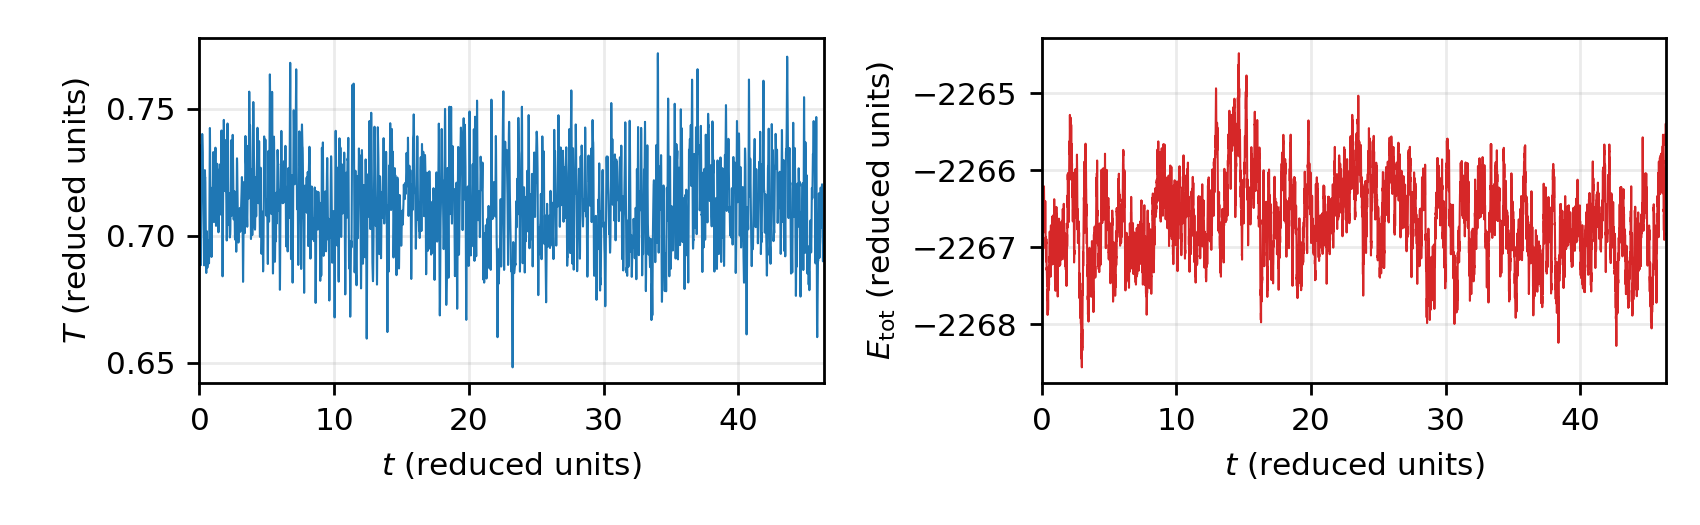
\includegraphics[width=0.85\linewidth]{../leapfrog_step1/md_results_plot.png}
  \caption{Temperature $T = 2E_{\text{kin}}/(3N-3)$ (left) and total truncated energy $E_{\text{tot}}$ (right), in reduced units.}
  \label{fig:ex1}
\end{figure}

\subsection{Discussion \& Notes}
\begin{itemize}
  \item \textbf{Energy:} leap-frog Verlet is symplectic, so $E_{\text{tot}}$ should only oscillate. We get $\langle E_{\text{tot}}\rangle = -2266.65$, and $\sigma_E = 0.537$ ($0.024\%$), a very small fluctuation.
  \item \textbf{Temperature:} $\langle T^*\rangle = 0.713$ ($85.4\text{ K}$), $\sigma_T = 0.0175$ ($2.5\%$). That is a much larger relative fluctuation than for $E_{\text{tot}}$, as $E_{\text{kin}}$ and $E_{\text{pot}}$ are exchanged. Both curves match the reference figures for a dense liquid.
\end{itemize}

\newpage
\section{Exercise 2}

\subsection{Question}
\paragraph{STEP 2: Analysing the structure and calculating thermodynamic properties.}
\begin{itemize}
  \item Modify the code to calculate the radial distribution function (RDF) $g(r)$ from the MD simulation. Compute the RDF for a run of $10000$ steps. Plot $g(r)$ vs.\ $r$ using reduced units.
  \item Modify the code to calculate the pressure $P$. Compute the mean values of the total and different contributions to $E$ and $P$. Include the tail corrections. Analyze the convergence of the results as a function of the simulation length. Use reduced units.
\end{itemize}

\subsection{Code}
Only the lines added for the radial distribution function, the virial pressure and the long-range tails are shown. The full program is listed in the Anex.

\lstinputlisting[style=fortranstyle,firstline=9,lastline=14,firstnumber=9,caption={Histogram storage. \texttt{nid} is real because a name starting with \texttt{n} would be an integer under implicit typing.},label={lst:ex2-decl}]{../leapfrog_step2/leapfroglj.f90}

\lstinputlisting[style=fortranstyle,firstline=49,lastline=62,firstnumber=49,caption={Tail corrections and zeroing of the RDF and pressure accumulators before the loop.},label={lst:ex2-init}]{../leapfrog_step2/leapfroglj.f90}

\lstinputlisting[style=fortranstyle,firstline=74,lastline=86,firstnumber=74,caption={Energy and pressure contributions accumulated on every step of the MD loop.},label={lst:ex2-loop}]{../leapfrog_step2/leapfroglj.f90}

\lstinputlisting[style=fortranstyle,firstline=92,lastline=97,firstnumber=92,caption={Run averages of the energy and pressure contributions.},label={lst:ex2-averages}]{../leapfrog_step2/leapfroglj.f90}

\lstinputlisting[style=fortranstyle,firstline=120,lastline=129,firstnumber=120,caption={Normalisation of $g(r)$ by the ideal-gas content of each shell.},label={lst:ex2-gr}]{../leapfrog_step2/leapfroglj.f90}

\lstinputlisting[style=fortranstyle,firstline=183,lastline=193,firstnumber=183,caption={Pair virial summed inside \texttt{forces}.},label={lst:ex2-forces}]{../leapfrog_step2/leapfroglj.f90}

\lstinputlisting[style=fortranstyle,firstline=230,lastline=237,firstnumber=230,caption={End of subroutine \texttt{lj}: virial of one pair inside the cutoff, and the $g(r)$ shell counted up to $L/2$.},label={lst:ex2-lj}]{../leapfrog_step2/leapfroglj.f90}

\subsection{Results}
The same $10000$-step trajectory as in Exercise~1 ($N = 500$, $\rho^* = 0.835$, $\langle T^*\rangle = 0.713$, $r_c = 2.5$) was used. $g(r)$ is accumulated in $1000$ shells up to $L^*/2 = 4.21$ and normalised by the ideal-gas content of each shell. The pressure is $P = P_{\text{kin}} + P_{\text{vir}} + P_{\text{tail}}$ with $P_{\text{kin}} = 2E_{\text{kin}}/(3V)$ and $P_{\text{vir}} = \frac{1}{3V}\sum_{i<j}\vec{r}_{ij}\cdot\vec{f}_{ij}$. The tails assume $g(r) = 1$ beyond $r_c$:
\begin{equation}
  E_{\text{tail}} = \frac{8\pi}{3}\rho N\left(\frac{1}{3r_c^9} - \frac{1}{r_c^3}\right) = -223.67, \qquad
  P_{\text{tail}} = \frac{16\pi}{3}\rho^2\left(\frac{2}{3r_c^9} - \frac{1}{r_c^3}\right) = -0.7465.
\end{equation}
Figure~\ref{fig:ex2} shows $g(r)$, the pressure contributions and the running means of the totals. Table~\ref{tab:ex2} gives the mean of every contribution after increasing simulation lengths. The last row is the full run.

\begin{figure}[H]
  \centering
  \begin{minipage}[t]{0.325\linewidth}
    \centering
    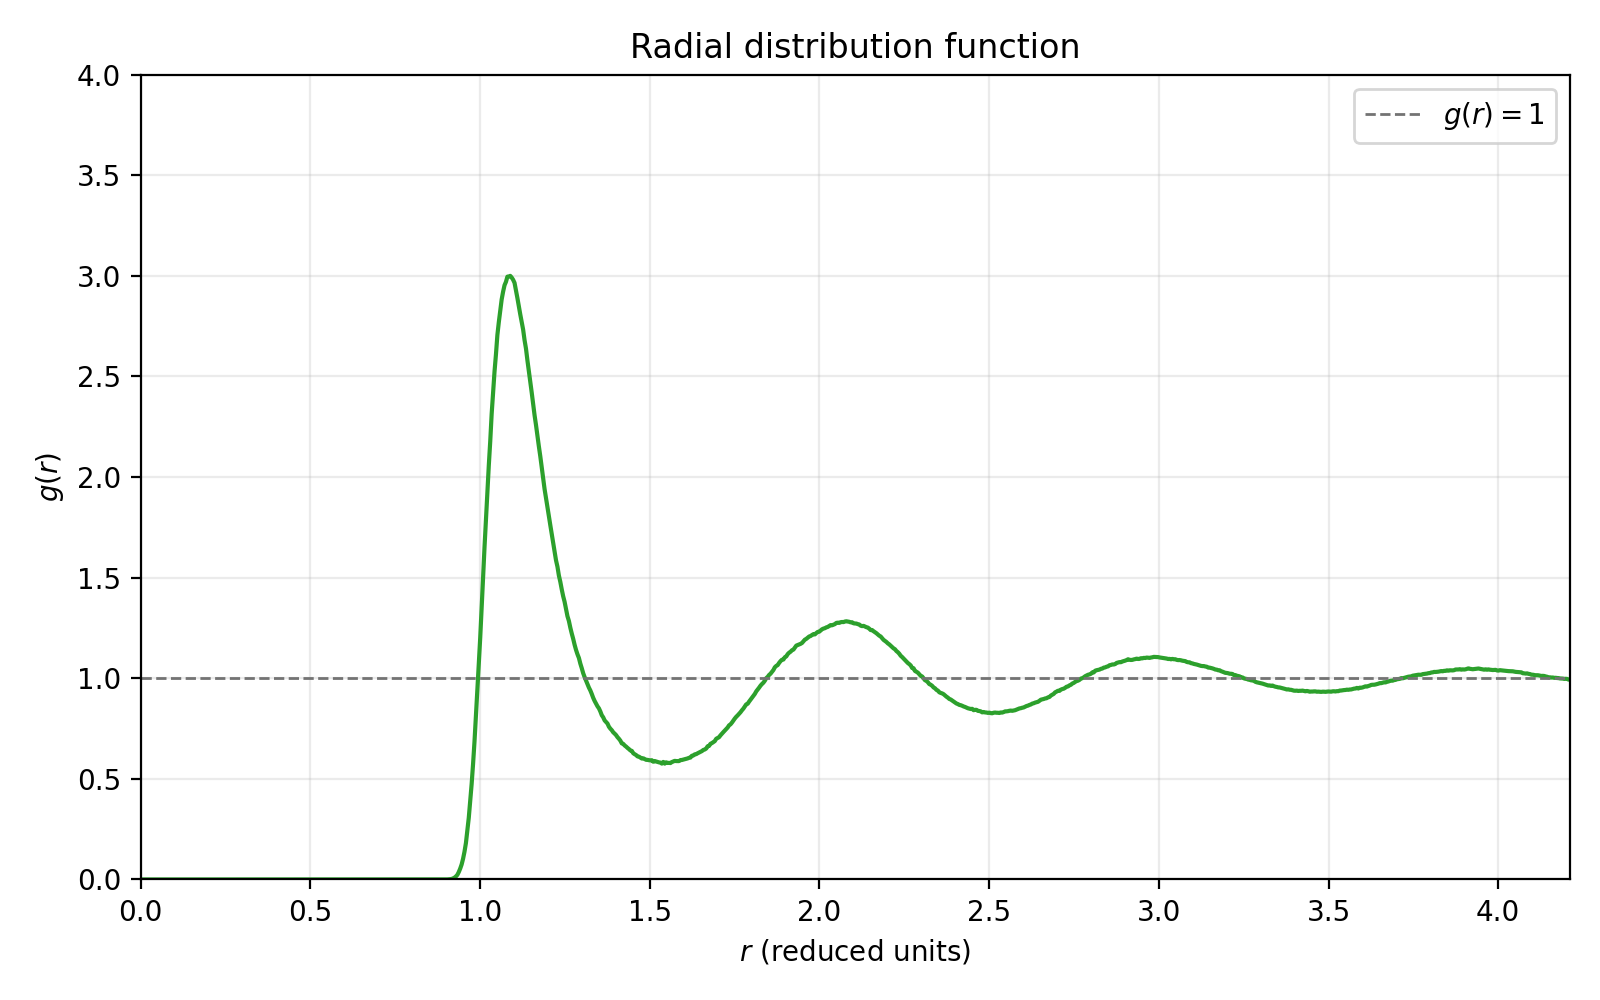
\includegraphics[width=\linewidth]{../leapfrog_step2/rdf_plot.png}\\[-2pt]
    {\small (a) RDF}
  \end{minipage}\hfill
  \begin{minipage}[t]{0.325\linewidth}
    \centering
    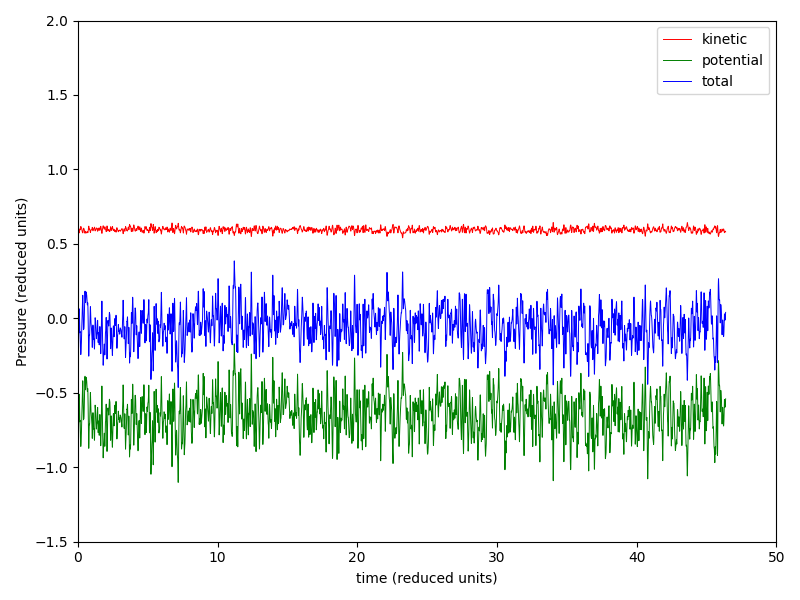
\includegraphics[width=\linewidth]{../leapfrog_step2/pressure_plot.png}\\[-2pt]
    {\small (b) Pressure}
  \end{minipage}\hfill
  \begin{minipage}[t]{0.325\linewidth}
    \centering
    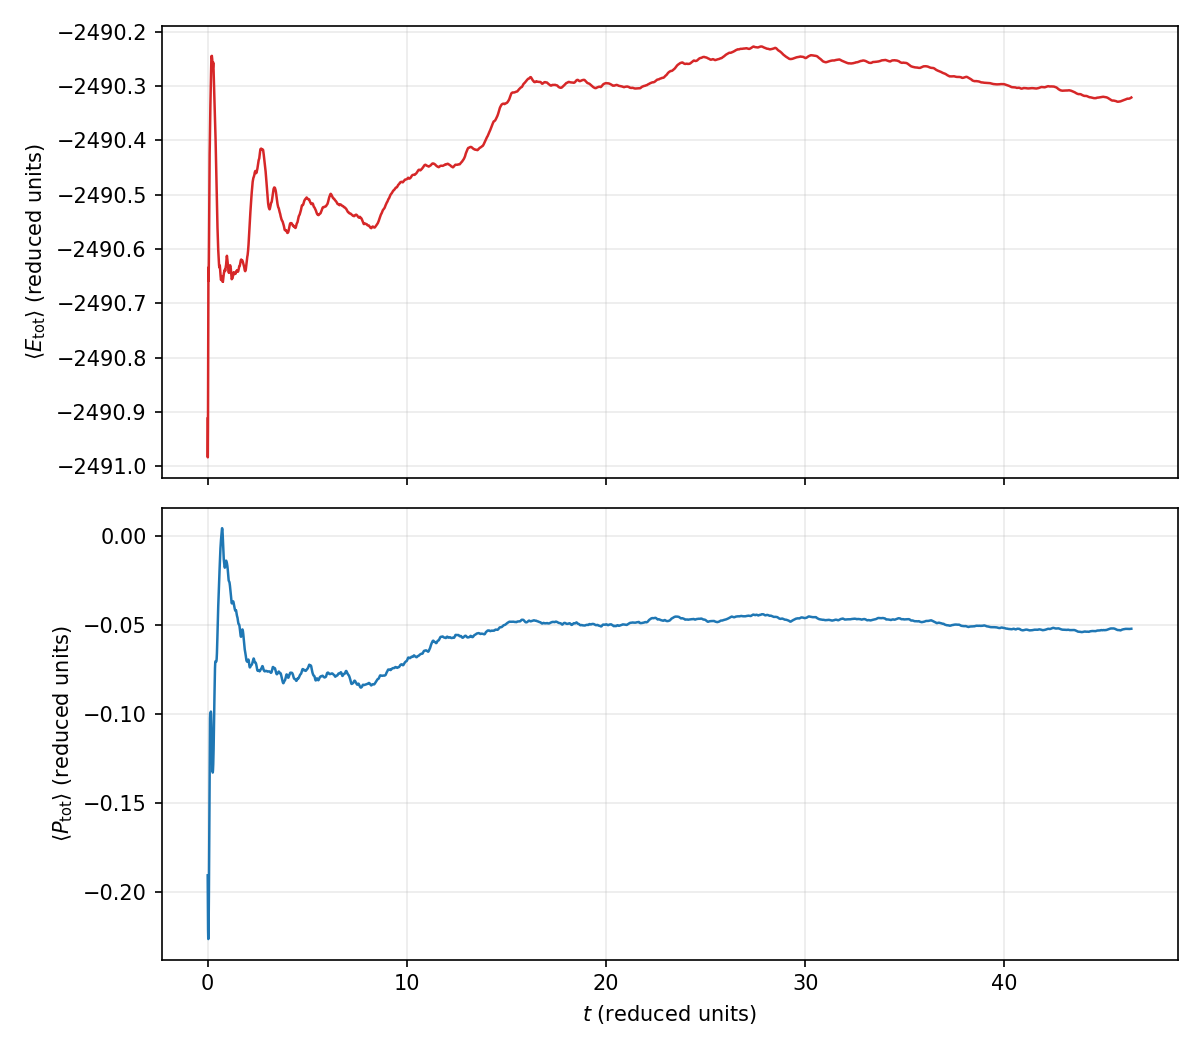
\includegraphics[width=\linewidth]{../leapfrog_step2/convergence_plot.png}\\[-2pt]
    {\small (c) Convergence}
  \end{minipage}
  \caption{Structure and thermodynamics of the Lennard-Jones liquid in reduced units. (a)~Radial distribution function $g(r)$. (b)~Kinetic, potential ($P_{\text{vir}} + P_{\text{tail}}$) and total pressure versus time. (c)~Running means of $E_{\text{tot}}$ and $P_{\text{tot}}$ (tails included) from $t = 0$ to $t$.}
  \label{fig:ex2}
\end{figure}

\begin{table}[H]
  \centering
  \small
  \caption{Mean energy and pressure contributions (reduced units) after $n$ steps. $E_{\text{tail}} = -223.67$ and $P_{\text{tail}} = -0.7465$ are constant and are included in the totals.}
  \label{tab:ex2}
  \begin{tabular}{rr|rrr|rrr}
    \hline
    $n$ & $t^*$ & $\langle E_{\text{kin}}\rangle$ & $\langle E_{\text{pot}}\rangle$ & $\langle E_{\text{tot}}\rangle$ & $\langle P_{\text{kin}}\rangle$ & $\langle P_{\text{vir}}\rangle$ & $\langle P_{\text{tot}}\rangle$ \\
    \hline
    1000  & 4.64  & 535.49 & $-2802.35$ & $-2490.53$ & 0.5965 & 0.0721 & $-0.0779$ \\
    2500  & 11.59 & 534.82 & $-2801.60$ & $-2490.45$ & 0.5958 & 0.0922 & $-0.0585$ \\
    5000  & 23.19 & 534.06 & $-2800.66$ & $-2490.27$ & 0.5949 & 0.1042 & $-0.0473$ \\
    7500  & 34.78 & 533.35 & $-2799.94$ & $-2490.26$ & 0.5941 & 0.1061 & $-0.0462$ \\
    10000 & 46.37 & 533.66 & $-2800.31$ & $-2490.32$ & 0.5945 & 0.1001 & $-0.0519$ \\
    \hline
  \end{tabular}
\end{table}

\subsection{Discussion \& Notes}
\begin{itemize}
  \item \textbf{RDF:} $g(r) = 0$ inside the repulsive core ($r \lesssim 0.93$) and then oscillates as in a dense liquid, matching the reference curve. The first peak is at $r = 1.089$ ($g = 3.00$), the first minimum at $r = 1.544$ ($g = 0.576$), and further peaks at $r = 2.079$ ($g = 1.28$) and $r = 2.985$ ($g = 1.11$). The oscillations die out and $g(L/2) = 0.993 \approx 1$: there is short-range order but no long-range order.
  \item \textbf{Energy:} $E_{\text{kin}}$ and $E_{\text{pot}}$ each fluctuate by $\sigma \approx 13$, in anti-phase, so their sum keeps the $\sigma = 0.537$ of Exercise~1. $\langle E_{\text{tot}}\rangle/N = -4.98$ per particle, and the tail is $9\%$ of $E_{\text{tot}}$.
  \item \textbf{Pressure:} $\langle P_{\text{kin}}\rangle = 0.5945 \approx \rho^* \langle T^*\rangle = 0.596$. The repulsive virial $0.100$ and the attractive tail $-0.746$ almost cancel it, so $P_{\text{tot}} = -0.052$ fluctuates around zero ($\sigma_P = 0.120$), as in the reference figure. Without the tail $P^*$ would be $+0.69$, so the tail correction is essential at $r_c = 2.5$.
  \item \textbf{Convergence:} $\langle E_{\text{tot}}\rangle$ changes by only $0.2$ (less than $0.01\%$) once a few thousand steps have been averaged. $\langle P_{\text{tot}}\rangle$ converges more slowly: it is a small difference of large terms, and its instantaneous fluctuations are more than twice its mean. It settles after about $5000$ steps ($t^* \approx 23$) to within $\pm 0.006$. Block averaging the full run (10 blocks) gives statistical errors of $0.07$ on $E_{\text{tot}}$ and $0.007$ on $P_{\text{tot}}$, so $10000$ steps are enough for both.
\end{itemize}

\newpage
\section{Exercise 3}

\subsection{Question}
\paragraph{STEP 3: Analysing the dynamics.}
\begin{itemize}
  \item Modify the code to calculate the velocity autocorrelation function (VACF) and the mean square displacement (MSD):
\begin{equation}
  C(t) = \bigl\langle \vec{v}(t)\cdot\vec{v}(0)\bigr\rangle,
\end{equation}
\begin{equation}
  r^{2}(t) = \bigl\langle \bigl[\vec{r}(t)-\vec{r}(0)\bigr]^{2}\bigr\rangle.
\end{equation}
  Compute the VACF and the MSD for a run of $10000$ steps. Plot the results.
  \item Write a code to calculate the spectral density (SDW) of the VACF:
\begin{equation}
  S(\omega) = \int_0^{\infty} dt\, C(t)\cos(\omega t).
  \label{eq:sdw}
\end{equation}
  Use a Simpson $3/8$ rule or similar. Plot the results.
  \item Use Einstein's diffusion formula to obtain the self-diffusion coefficient $D$:
\begin{equation}
  D = \lim_{t\to\infty}\frac{1}{6t}\, r^{2}(t).
  \label{eq:einstein}
\end{equation}
\end{itemize}

\subsection{Code}
Only the lines added in this step are shown, with a few lines of the existing program kept where they mark the insertion point. The full program is listed in the Anex.

\lstinputlisting[style=fortranstyle,firstline=11,lastline=21,firstnumber=11,caption={Unwrapped-trajectory arrays \texttt{runw}, \texttt{rold}, and storage for the VACF, the MSD, the spectral density and the time-origin buffers.},label={lst:ex3-decl}]{../leapfrog_step3/leapfroglj.f90}

\lstinputlisting[style=fortranstyle,firstline=51,lastline=56,firstnumber=51,caption={Unwrapped coordinates, initialised once the positions are in reduced units.},label={lst:ex3-runw}]{../leapfrog_step3/leapfroglj.f90}

\lstinputlisting[style=fortranstyle,firstline=74,lastline=90,firstnumber=74,caption={Correlation window and circular buffer of time origins.},label={lst:ex3-window}]{../leapfrog_step3/leapfroglj.f90}

\lstinputlisting[style=fortranstyle,firstline=99,lastline=110,firstnumber=99,caption={Each leap-frog step is unfolded before \texttt{sample} accumulates $C(t)$ and $r^{2}(t)$.},label={lst:ex3-unfold}]{../leapfrog_step3/leapfroglj.f90}

\lstinputlisting[style=fortranstyle,firstline=169,lastline=198,firstnumber=169,caption={Normalisation and output of the VACF and the MSD, and spectral density of $C(t)$.},label={lst:ex3-vacf}]{../leapfrog_step3/leapfroglj.f90}

\lstinputlisting[style=fortranstyle,firstline=208,lastline=227,firstnumber=208,caption={Einstein self-diffusion coefficient from a linear fit of $r^{2}(t)$ in the diffusive regime.},label={lst:ex3-diff}]{../leapfrog_step3/leapfroglj.f90}

\lstinputlisting[style=fortranstyle,firstline=253,lastline=309,firstnumber=253,caption={Internal subroutine \texttt{sample}: VACF and MSD with multiple time origins.},label={lst:ex3-sample}]{../leapfrog_step3/leapfroglj.f90}

\lstinputlisting[style=fortranstyle,firstline=311,lastline=347,firstnumber=311,caption={Internal subroutine \texttt{spectrum}: composite Simpson $3/8$ cosine transform of the VACF.},label={lst:ex3-spectrum}]{../leapfrog_step3/leapfroglj.f90}

\subsection{Results}
On the same $10000$-step trajectory ($N = 500$, $\rho^* = 0.835$, $\langle T^*\rangle = 0.713$), $C(t)$ and $r^{2}(t)$ were averaged over particles and time origins in a window of $1074$ steps ($t^* \le 4.98$). Figure~\ref{fig:ex3} shows the VACF, the MSD with its Einstein fit, and the spectral density $S(\omega)$. The fit gives a slope of $0.1988$ and an intercept of $0.025$, so $D^* = 0.0331$, i.e.\ $D = D^*\sigma^2/\tau = 0.178\text{ \AA}^2\text{ ps}^{-1} = 1.78\times 10^{-5}\text{ cm}^2\text{ s}^{-1}$.

\begin{figure}[H]
  \centering
  \begin{minipage}[t]{0.325\linewidth}
    \centering
    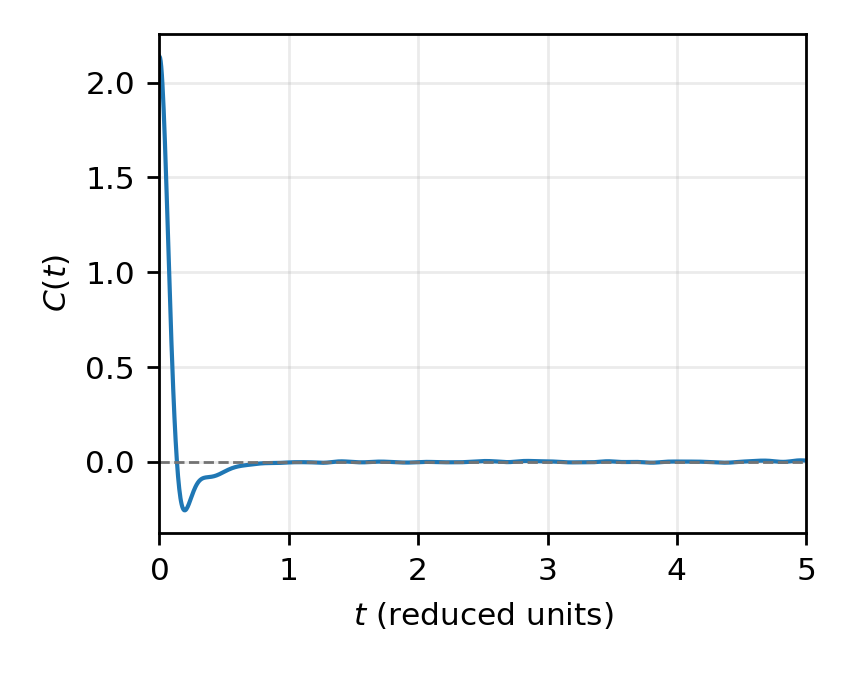
\includegraphics[width=\linewidth]{../leapfrog_step3/vacf_plot.png}\\[-2pt]
    {\small (a) VACF}
  \end{minipage}\hfill
  \begin{minipage}[t]{0.325\linewidth}
    \centering
    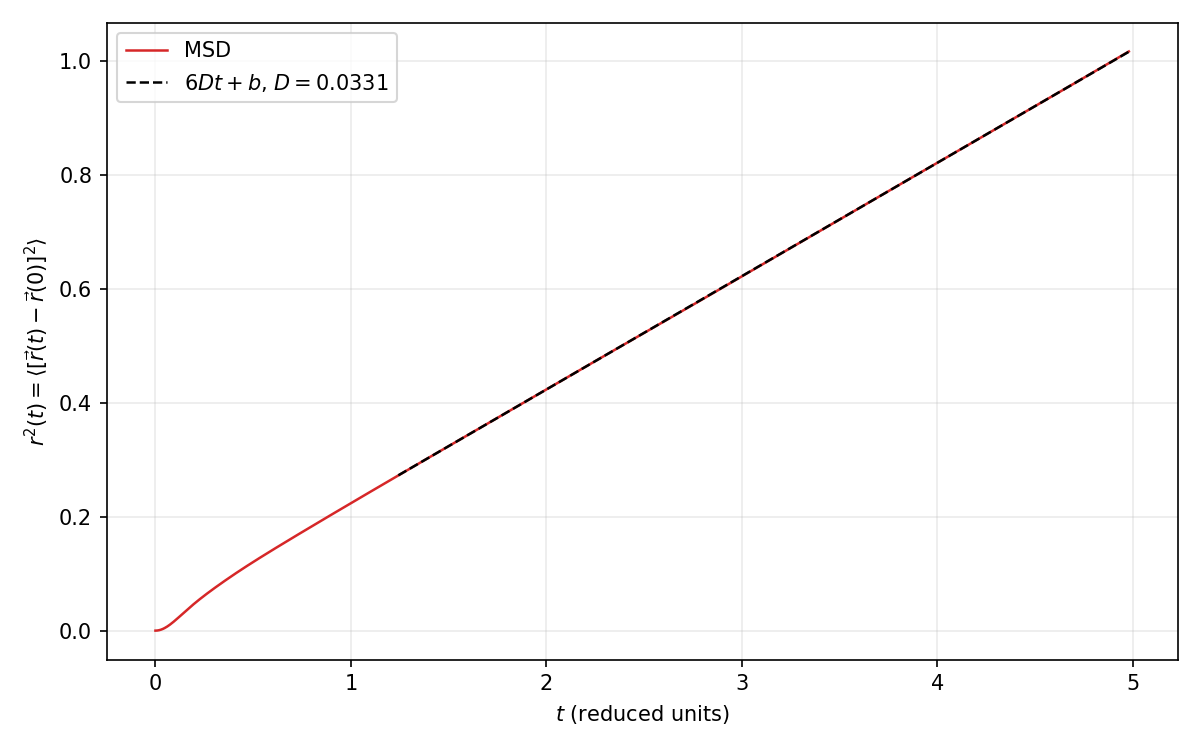
\includegraphics[width=\linewidth]{../leapfrog_step3/msd_plot.png}\\[-2pt]
    {\small (b) MSD}
  \end{minipage}\hfill
  \begin{minipage}[t]{0.325\linewidth}
    \centering
    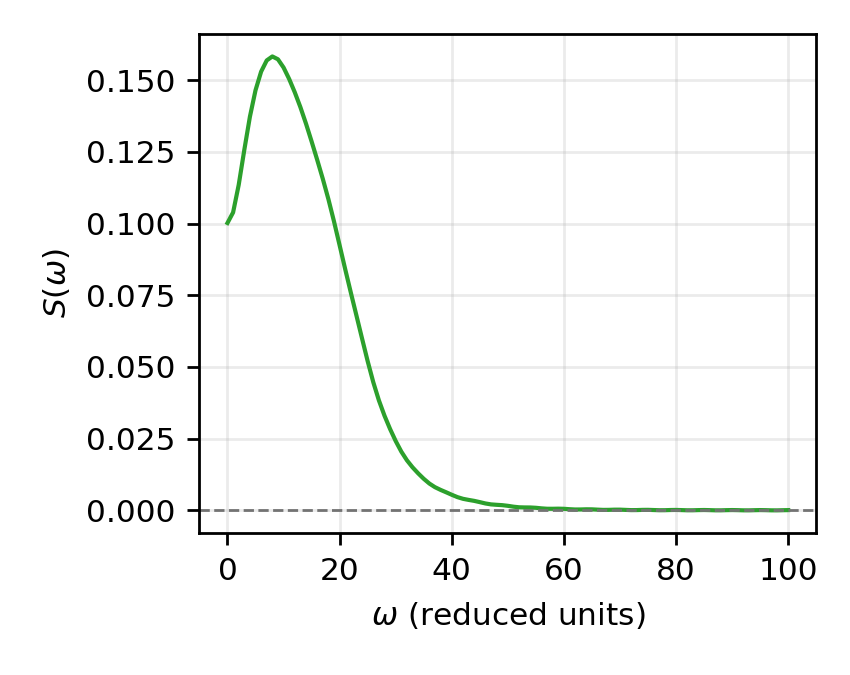
\includegraphics[width=\linewidth]{../leapfrog_step3/sdw_plot.png}\\[-2pt]
    {\small (c) SDW}
  \end{minipage}
  \caption{Dynamics of the Lennard-Jones liquid in reduced units. (a)~Velocity autocorrelation $C(t)$. (b)~Mean square displacement $r^{2}(t)$; the dashed line is the fit $r^{2} = 6Dt + b$ on $t^* \in [1.24, 4.98]$. (c)~Spectral density $S(\omega)$ of the VACF, Simpson $3/8$ rule, $\omega = 0,1,\ldots,100$.}
  \label{fig:ex3}
\end{figure}

\subsection{Discussion \& Notes}
\begin{itemize}
  \item \textbf{Method and setup:}
  Following the lecture SAMPLE scheme, a new time origin is stored every $5$ steps in a circular buffer. The MSD uses unwrapped positions: each leap-frog displacement is unfolded with the minimum image, so $r^{2}(t)$ is not folded back by the periodic box. The window $n_{\text{cor}} = 1074$ is a multiple of $6$, so Simpson's $3/8$ rule has complete panels, and it is long enough for $C(t)$ to vanish and for $r^{2}(t)$ to become linear. The integral~\eqref{eq:sdw} is evaluated on $t^* \le 1.24$ (first quarter of the window), beyond which $C(t)\approx 0$. Following~\eqref{eq:einstein}, $D$ is one sixth of the slope of $r^{2}(t)$ fitted over the last three quarters of the window, which discards the ballistic rise.

  \item \textbf{Results vs expectations:}
  \begin{itemize}
    \item \emph{VACF:} $C(0) = 2.138$ agrees with the equipartition value $\langle v^2\rangle = 3\langle T^*\rangle = 2.139$ ($m = 1$). $C(t)$ decays quickly, crosses zero at $t^* = 0.139$ and reaches a minimum $C = -0.256$ at $t^* = 0.195$. This negative lobe is the signature of a dense liquid: atoms rebound from the cage of first neighbours (the RDF peak at $r = 1.09$ in Exercise~2). Beyond $t^* \approx 0.64$, $\vert C\vert < 0.02$ and $C(t)$ only fluctuates around zero.
    \item \emph{MSD:} $r^{2}(t)$ follows the ballistic law $\langle v^2\rangle t^2$ only for $t^* \lesssim 0.05$ ($r^2 = 0.0053$ against $0.0056$), bends as collisions set in, and is linear for $t^* \gtrsim 1$. It reaches $r^{2} = 1.016$ at $t^* = 4.98$, so each atom moves about one $\sigma$ in the window.
    \item \emph{SDW:} $S(\omega)$ peaks at $\omega = 8$ ($S = 0.158$), the characteristic frequency of an atom rattling in its cage and the counterpart of the negative VACF lobe. It falls to $5.4\times 10^{-3}$ at $\omega = 40$ and $5\times 10^{-5}$ at $\omega = 100$, so no motion is faster than the collision time. $S(0) = 0.100$ is finite, as it must be for a fluid (a solid has $S(0) = 0$), and $S(0)/3 = 0.0334$ matches the Einstein $D^*$ to $1\%$.
    \item \emph{Self-diffusion:} $D = 1.78\times 10^{-5}\text{ cm}^2\text{ s}^{-1}$ is of the order expected for simple liquids near their triple point.
  \end{itemize}

  \item \textbf{Conclusion:}
  A window of $5$ reduced time units suffices: the VACF has died out and the MSD is linear. The cage-backscattering lobe of $C(t)$, the peak of $S(\omega)$ at $\omega = 8$ and $D^* = 0.033$ all describe a dense Lennard-Jones liquid, consistent with the RDF of Exercise~2.
\end{itemize}

\clearpage
\thispagestyle{empty}
\null
\vspace*{\fill}
\begin{center}
{\fontsize{48}{58}\selectfont\bfseries Anex}
\end{center}
\vspace*{\fill}
\clearpage
The program listed here is the full source used throughout the practice. It is the leap-frog integrator supplied for Exercise~1, together with the radial distribution function, the virial pressure and the tail corrections added in Exercise~2, and the velocity autocorrelation, mean square displacement, spectral density and self-diffusion coefficient added in Exercise~3. Each exercise section quotes only the lines introduced in that step.

\lstinputlisting[style=fortranstyle,caption={Full leap-frog program used for the three exercises.},label={lst:ex3}]{../leapfrog_step3/leapfroglj.f90}
\end{document}
